\documentclass{lab}

\newcommand{\R}{R_{_{\sum}}}

\begin{document}

\begin{titlepage}

\pagestyle{empty}	% Нумерация выкл.

\begin{center}
	\textsc{\LARGE Московский Физико-Технический Институт}\\[1,5cm]
	\textsc{\Large Кафедра общей физики}\\[0,5cm]
	\textsc{\large Лабораторная работа \textnumero 3.4.2}\\[2.5cm]

	\noindent\rule{\textwidth}{1pt}
	\\[0.5cm]
	{ \huge \bfseries Закон Кюри-Вейсса}
	\\[0.1cm]
	\noindent\rule{\textwidth}{1pt}
\end{center}

\vfill

\begin{minipage}[b]{0.3\textwidth}
	Маршрут \RomanNumeralCaps{3}\\\\
	20 октября 2018 г.\\
	27 октября 2018 г.
\end{minipage}
\hfill
\begin{minipage}[b]{0.33\textwidth}
	\textit{Работу выполнил}\\
	Ринат Валиев, 711 гр.\\\\
	\textit{Под руководством}\\
	Г.И. Лапушкина, к.ф.-м.н.
\end{minipage}

\end{titlepage}

\pagestyle{VR}
\setcounter{page}{2}

\section*{Постановка эксперимента}

\begin{quote}
\textbf{{\normalsize Цель работы: }}
исследование резонанса напряжений в последовательном колебательном контуре с
изменяемой емкостью, включающее получение амплитудно-частотных и фазово-частотных
характеристик, а также определение основных параметров контура.
\end{quote}

\begin{quote}
\textbf{{\normalsize Оборудование: }}
генератор сигналов, источник напряжения, нагруженный на последовательный колебательный
контур с переменной емкостью, двулучевой осциллограф, цифровые вольтметры.
\end{quote}

\subsection*{Теоретическая часть}

Схема экспериментального стенда для изучения резонанса напряжений в последовательном
колебательном контуре показана на рис. \ref{setup}. Синусоидальный сигнал от генератора
$GFG8255A$ поступает через согласующую $RC$-цепочку на вход источника напряжения,
собранного на операционном усилителе ОУ. Источник напряжения, обладающий по определению
нулевым внутренним сопротивлением, фактически обеспечивает с высокой точностью
постоянство амплитуды сигнала $ E = E_0 \cos (\omega t + \varphi_0) $ на меняющейся по
величине нагрузке -- последовательном колебательном контуре, изображенном на
рис. \ref{setup} в виде эквивалентной схемы. Источник напряжения с согласующей цепочкой,
колебательный контур и блок питания заключены в отдельный корпус с названием
«Резонанс напряжений», отмеченный на рисунке штриховой линией.

\begin{figure}[H]
	\centering
	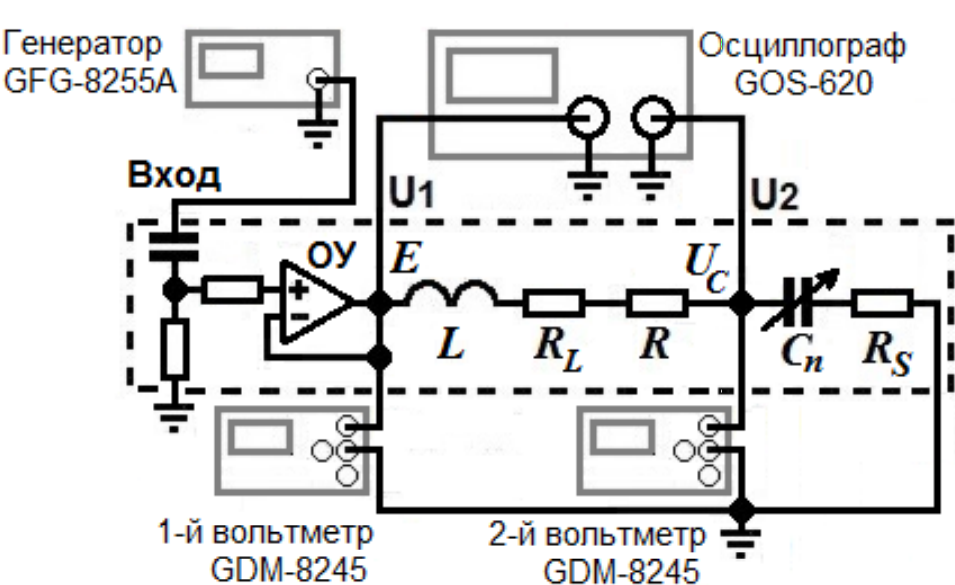
\includegraphics[width = 0.7 \textwidth]{setup}
	\caption{\footnotesize
	Схема экспериментальной установки для исследования резонанса напряжений
	}
	\label{setup}
\end{figure}

В нашем контуре катушка индуктивности $ L $ на ферритовом каркасе обладает малым
сопротивлением по постоянному току и высокой собственной частотой
$ f_r\,\geq\,1.3 МГц$. В общем случае индуктивность $ L_{eff} = L/(1-f^2/f_r^2) $,
но у нас $ f \ll f_r $, так что $ L_{eff} = L $.\\

\begin{wrapfigure}[10]{l}{5cm}
	\vspace{-0.5cm}
	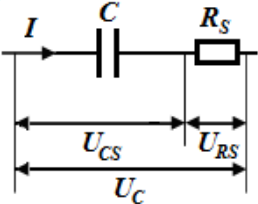
\includegraphics[width=5cm]{capacitor}
	\caption{\footnotesize
	Последовательная эквивалентная схема конденсатора с потерями
	}
	\label{capacitor}
\end{wrapfigure}

Конденсаторы, конечно, тоже не идеальные. $ R_S $ -- эквивалентное последовательное
сопротивление (ЭПС), обусловленное электрическим сопротивлением материала обкладок,
выводов, контактов, потерями в диэлектрике. Тогда, учитывая сдвиг фаз -- $ \varphi $:

$$ R_S = \dfrac{U_{RS}}{I} = \dfrac{U_{RS}}{\omega CU_{CS}} = \dfrac{1}{\omega C}
\tan \delta, ~~~~~ где ~ \delta = \pi / 2 - \varphi $$

В нашем эксперименте $ \tan \delta < 10^{-3} $ -- хороший показатель для конденсатора
с твердым диэлектриком.\\

Активное сопротивление в итоге: $ \R = R + R_L + R_S $, далее будем пользоваться
методом комплексных амплитуд. Получаем импедансы:

$$ Z_L = R_L + i \omega L, ~~~~~ Z_C = R_S - i\dfrac{1}{\omega C}, ~~~~~ Z = \R +
i \left(\omega L - \dfrac{1}{\omega C}\right) $$ 

В работе используются стандартные обозначения: $ \omega_0 = 1/\sqrt{LC} $ -- собственная
частота из условия $ \Im Z = 0 $, $ \rho = \sqrt{L/C} $ -- реактивное сопротивление
контура, Q -- добротность колебательного контура:

$$ Q = \rho / \R = \omega_0 L / \R = 1 / \omega_0 C \R \gg 1 $$

При данном условии $ \omega_0 $ называют резонансной частотой. Также наибольший интерес
представляет случай $ \abs{\Delta \omega} \ll \omega_0 $:

$$ \dfrac{\omega}{\omega_0} - \dfrac{\omega_0}{\omega} = \dfrac{2\Delta\omega}{\omega_0} $$

Используя этот факт, можем выразить добротность контура через ширину резонансной кривой:

\begin{equation}
\begin{aligned}
&\dfrac{I_0}{I_{0,~рез}} = \dfrac{1}{\sqrt{1 + Q^2 \left(\dfrac{\omega_0}{\omega} -
		\dfrac{\omega}{\omega_0}\right)^2}}\\
&\dfrac{I_0}{I_{0,~рез}} = \dfrac{1}{\sqrt{1 +
		Q^2 \left(\dfrac{2\Delta\omega}{\omega_0}\right)^2}}\\
&Q = \dfrac{\omega_0}{2\Delta\omega} ~~~~~~~ при ~ \dfrac{I_0}{I_{0,~рез}} =
		\dfrac{1}{\sqrt{2}}
\end{aligned}
\end{equation}

\newpage

\section*{Выполнение эксперимента}

\subsection*{Измерения}

\vspace{0.5cm}

\begin{enumerate}

\item
Настроим оборудование и приступим к работе. Для контуров с 7 различными $ C_n $ измерим
резонансные частоты $ f_{0} $ и напряжения $ U_C(f_{0}) $ и $ E(f_{0}) $.
Резонанс легче ловить по фигурам Лисажу.

\begin{table}[H]
	\centering
	\begin{tabular}{|c|ccccccc|}
		\hline
		$n$			&1		&2		&3		&4		&5		&6		&7		\\ \hline
		$C_n, нФ$	&24,8	&32,3	&47,6	&57,5	&68,0	&81,6	&102,8	\\ %\hline
		$f_0, кГц$	&32,05	&27,72	&23,17	&21,08	&19,39	&17,70	&15,77	\\ %\hline
		$U_C, В$	&7,30	&6,57	&5,69	&5,26	&4,89	&4,54	&4,11	\\ %\hline
		$E, В$		&0,3	&0,3	&0,3	&0,3	&0,3	&0,3	&0,3	\\ \hline
	\end{tabular}
	\caption{\footnotesize 
	Резонансные частоты $ f_{0} $ для контуров с разными емкостями $ C_n $, также
	напряжения на конденсаторе $ U_C(f_{0}) $ и в контуре $ E(f_{0}) $
	(рис. \ref{setup}) для каждого случая
	}
	\label{tab0}
\end{table}

\vspace{0.7cm}

\item
Для контуров с двумя различными емкостями снимем данные для АЧХ $ U_C(f) $ при том же напряжении $ E = 0.3~В$.

\begin{table}[H]
	{\small 
	\begin{tabular}{|c|c|ccccccccccc|}
		\hline
		\multirow{8}{*}{$С_2$}
		&$f, кГц$		&16,73	&17,71	&18,68	&19,93	&20,53	&22,09	&23,06	&24,45	&25,24	&26,65	&27,57	\\
		&$U_C, В$		&0,470	&0,503	&0,543	&0,610	&0,650	&0,791	&0,927	&1,250	&1,578	&3,143	&6,431	\\
		&$f/f_{рез}$	&0,60	&0,64	&0,67	&0,72	&0,74	&0,80	&0,83	&0,88	&0,91	&0,96	&0,99	\\
		&$U/U_{рез}$	&0,07	&0,08	&0,08	&0,09	&0,10	&0,12	&0,14	&0,19	&0,24	&0,48	&0,98	\\ \cline{2-13}
		&$f, кГц$		&27,72	&28,37	&29,44	&30,35	&31,38	&32,33	&33,68	&35,22	&36,44	&37,97	&38,72	\\
		&$U_C, В$		&6,570	&4,752	&2,456	&1,636	&1,156	&0,898	&0,678	&0,523	&0,437	&0,362	&0,333	\\
		&$f/f_{рез}$	&1,00	&1,02	&1,06	&1,09	&1,13	&1,17	&1,22	&1,27	&1,31	&1,37	&1,40	\\
		&$U/U_{рез}$	&1,00	&0,72	&0,37	&0,25	&0,18	&0,14	&0,10	&0,08	&0,07	&0,06	&0,05	\\ \hline
	\end{tabular}
\\[1pt]
	\begin{tabular}{|c|c|ccccccccc|}
		\hline
		\multirow{8}{*}{$С_6$}
		&$f, кГц$		&10,64	&11,58	&12,25	&13,52	&14,60	&15,57	&16,21	&17,06	&17,52	\\
		&$U_C, В$		&0,466	&0,518	&0,566	&0,698	&0,888	&1,213	&1,632	&3,050	&4,350	\\
		&$f/f_{рез}$	&0,60	&0,65	&0,69	&0,76	&0,82	&0,88	&0,92	&0,96	&0,99	\\
		&$U/U_{рез}$	&0,10	&0,11	&0,12	&0,15	&0,20	&0,27	&0,36	&0,67	&0,96	\\ \cline{2-11}
		&$f, кГц$		&17,70	&18,17	&19,11	&20,08	&20,94	&21,79	&22,60	&23,76	&24,40	\\
		&$U_C, В$		&4,540	&3,620	&1,815	&1,100	&0,797	&0,620	&0,505	&0,397	&0,353	\\
		&$f/f_{рез}$	&1,00	&1,03	&1,08	&1,13	&1,18	&1,23	&1,28	&1,34	&1,38	\\
		&$U/U_{рез}$	&1,00	&0,80	&0,40	&0,24	&0,18	&0,14	&0,11	&0,09	&0,08	\\ \hline
	\end{tabular}
	}
	\caption{\footnotesize 
	Зависимость напряжения на конденсаторе $ U_C $ от частоты подаваемого сигнала для емкостей
	$ C_2 $ и $ C_6 $, а также приведенные частота и напряжение для дальнейшего использования
	при построении графика АЧХ
	}
	\label{tabAFC}
\end{table}

\newpage

\item
Построим график АЧХ $ U_C(f) $ в приведенных координатах (значения в таблице \ref{tabAFC})
при напряжении $ E = 0.3~В $ для емкостей $ C_2 $ и $ C_6 $:

\begin{figure}[H]
	\centering
	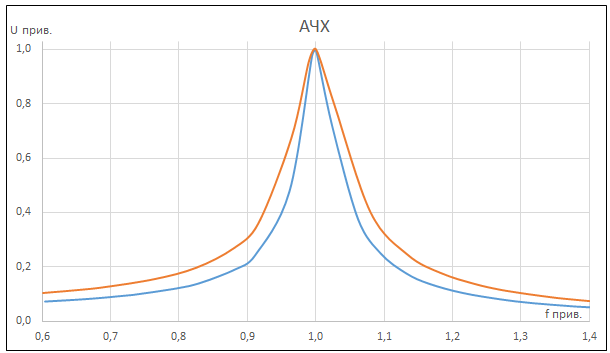
\includegraphics[width = \textwidth]{AFC}
	\caption{\footnotesize
	График АЧХ напряжения $ U_C(f) $ для контуров с конденсаторами $ C_2 $ и $ C_6 $
	при одном напряжении $ E = 0.3~В $ в приведенных координатах (таб. \ref{tabAFC})
	(широкая $ \longrightarrow для \ C_6 $)
	}
	\label{AFC}
\end{figure}

\item
Для тех же двух контуров снимем ФЧХ $ \varphi_C(f) $ при том же напряжении $ E~=~0.3~В $.

\end{enumerate}

\begin{wrapfigure}[8]{R}{9cm}
	\vspace{-1.2cm}
	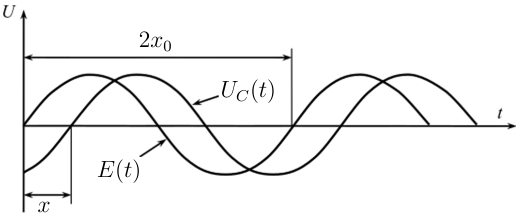
\includegraphics[width=9cm]{phi}
	\caption{\footnotesize Осциллограммы сигналов $ E(t) $ и $ U_C(t) $}
	\label{phi}
\end{wrapfigure}

\vspace{0.4cm}

Расстояние $ x $ от начала отсчета до точки первого обращения в нуль напряжения $ U_C(t) $,
которое показано на рисунке \ref{phi}, характеризует разность фаз
$ \Delta\varphi~=~(x/x_0)\pi $.\\ \\ \\
Результаты измерений для ФЧХ с конденсатором $ C_2 $:

\begin{table}[H]
	\centering
	{
		\begin{tabular}{|c|c|ccccccc|}
			\hline
			\multirow{6}{*}{$С_2$}
			&$ f, кГц $		&	16,40	&	22,72	&	25,00	&	25,38	&	26,00	&	26,35	&	27,00	\\
			&$ x/x_0 $		&	0,00	&	0,05	&	0,08	&	0,08	&	0,11	&	0,13	&	0,21	\\
			&$ f/f_{рез} $	&	0,59	&	0,82	&	0,90	&	0,92	&	0,94	&	0,95	&	0,97	\\ \cline{2-9}
			&$ f, кГц $		&	27,44	&	27,77	&	28,26	&	28,60	&	29,40	&	31,57	&	35,00	\\
			&$ x/x_0 $		&	0,37	&	0,53	&	0,70	&	0,78	&	0,88	&	0,94	&	1,00	\\
			&$ f/f_{рез} $	&	0,99	&	1,00	&	1,02	&	1,03	&	1,06	&	1,14	&	1,26	\\ \hline
		\end{tabular}
	}
	\caption{\footnotesize
	Сдвиг фаз $ \left(\varphi\pi = x/x_0\right) $ в зависимости от частоты сигнала $ f $ для
	контура	с конденсатором $ C_2 $, также приведенная частота для дальнейшего использования при
	построении графика ФЧХ
	}
	\label{tabPFC2}
\end{table}

\newpage

Результаты измерений для ФЧХ с конденсатором $ C_6 $:

\begin{table}[H]
	\centering
	{
		\begin{tabular}{|c|c|cccccccc|}
			\hline
			\multirow{6}{*}{$С_6$}
			&$ f, кГц $		&	12,80	&	14,44	&	15,66	&	16,29	&	16,56	&	16,99	&	17,09	&	17,46	\\
			&$ x/x_0 $		&	0,00	&	0,03	&	0,06	&	0,13	&	0,17	&	0,21	&	0,24	&	0,38	\\
			&$ f/f_{рез} $	&	0,72	&	0,82	&	0,88	&	0,92	&	0,94	&	0,96	&	0,97	&	0,99	\\ \cline{2-10}
			&$ f, кГц $		&	17,53	&	17,77	&	18,28	&	18,67	&	19,10	&	20,10	&	22,85	&	27,00	\\
			&$ x/x_0 $		&	0,41	&	0,54	&	0,74	&	0,81	&	0,88	&	0,92	&	0,95	&	1,00	\\
			&$ f/f_{рез} $	&	0,99	&	1,00	&	1,03	&	1,05	&	1,08	&	1,14	&	1,29	&	1,53	\\ \hline
		\end{tabular}
	}
	\caption{\footnotesize
	Сдвиг фаз $ \left(\varphi\pi = x/x_0\right) $ в зависимости от частоты сигнала $ f $ для
	контура	с конденсатором $ C_6 $, также приведенная частота для дальнейшего использования при
	построении графика ФЧХ
	}
	\label{tabPFC6}
\end{table}

\begin{enumerate}

\setcounter{enumi}{4}		%	!!!!!	!!!!!	!!!!!	костыль

\item
Построим график ФЧХ $ \varphi(f) $ в приведенных координатах (данные из таблиц \ref{tabPFC2} и
\ref{tabPFC6}) при напряжении $ E = 0.3~В $ для емкостей $ C_2 $ и $ C_6 $:

\begin{figure}[H]
	\centering
	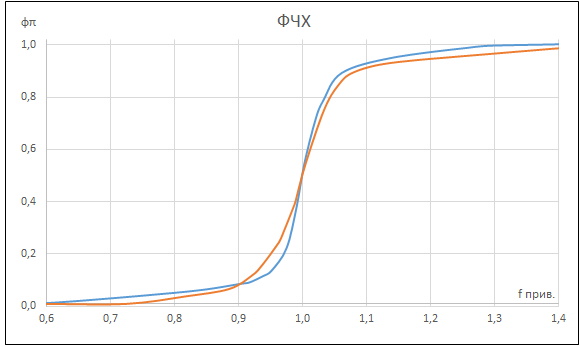
\includegraphics[width = \textwidth]{PFC}
	\caption{\footnotesize
	График ФЧХ $ \varphi(f) $ для контуров с конденсаторами $ C_2 $ и $ C_6 $
	при одном напряжении $ E = 0.3~В $ в приведенных координатах
	(таб. \ref{tabPFC2} и \ref{tabPFC6})\\
	(С меньшим углом наклона около $ f_{прив} = 1 \longrightarrow $~для~$ C_6 $)
	}
	\label{PFC}
\end{figure}

\end{enumerate}

\subsubsection*{Замечание}

На графиках \ref{AFC} и \ref{PFC} не показаны погрешности, т.к. они настолько малы, что кресты
не были бы видны. К примеру: погрешность показаний вольтметра всего лишь 1 мВ, в то время как
наименьший результат измерения 300 мВ. Подробнее погрешности разобраны ниже.

\newpage

\subsection*{Обработка данных}

\begin{enumerate}

\item
Для нахождения интересующих нас величин будут хорошо знакомые нам из теоретической части работы
формулы:

\begin{equation}
\begin{aligned}
&L = \dfrac{1}{\left(2 \pi f\right)^2C}; ~~~~~~~ Q = \dfrac{U_{C, рез}}{E}; ~~~~~~~
\rho = \sqrt{\dfrac{L}{C}}; ~~~~~~~ \R = \dfrac{\rho}{Q};\\
&R_S = \dfrac{1}{2 \pi f C} \cdot \tan \delta < \dfrac{1}{2 \pi f C} \cdot 10^{-3}; ~~~~~~~
R_L = \R - R - R_S\\
\end{aligned}
\end{equation}

Результаты измерений и вычислений внесем в таблицу:

\begin{table}[H]
\centering
{
\begin{tabular}{|cccc|cccccc|}
\hline
$ C_n,~нФ $	&$ f_0,~кГц $	&$ U_C,~В $	&$ E,~В $	&$ L,~мкГн $&$ Q $		&$ \rho,~Ом $	&$ \R,~Ом $	&$ R_S,~Ом $	&$ R_L,~Ом $\\ \hline
24,8		&	32,1		&	7,30	&	0,3		&	994		&	24,3	&	200			&	8,2		&	0,20		&	4,5		\\
32,3		&	27,7		&	6,57	&	0,3		&	1021	&	21,9	&	178			&	8,1		&	0,18		&	4,4		\\
47,6		&	23,2		&	5,69	&	0,3		&	991		&	19,0	&	144			&	7,6		&	0,14		&	4,0		\\
57,5		&	21,1		&	5,26	&	0,3		&	991		&	17,5	&	131			&	7,5		&	0,13		&	3,9		\\
68,0		&	19,4		&	4,89	&	0,3		&	991		&	16,3	&	121			&	7,4		&	0,12		&	3,8		\\
81,6		&	17,7		&	4,54	&	0,3		&	991		&	15,1	&	110			&	7,3		&	0,11		&	3,7		\\
102,8		&	15,8		&	4,11	&	0,3		&	991		&	13,7	&	98			&	7,2		&	0,10		&	3,6		\\ \hline
\multicolumn{4}{|l|}{Среднее значение}				&	996		&	\multicolumn{4}{c}{}								&	4,0		\\
\multicolumn{4}{|l|}{Среднекв. погрешность}			&	4,2		&	\multicolumn{4}{c}{}								&	0,1		\\
\multicolumn{4}{|l|}{Максимальное отклонение}		&	0,1		&	0,1		&	0,01		&	0,05	&$3\cdot10^{-5}$&	0,1		\\
\multicolumn{4}{|l|}{Абсолютная погрешность}		&	4,2		&	\multicolumn{4}{c}{}								&	0,2		\\
\multicolumn{4}{|l|}{Относительная погрешность}		&	0,4\%	&	\multicolumn{4}{c}{}								&	4\%		\\ \hline
\end{tabular}
}
\caption{\footnotesize
Основные характеристики каждого контура с различными емкостями конденсаторов~$ C_n $ и
падениями напряжения $ U_C $\\
Пояснения к величинам даны сверху, также в теоретической части работы.
}
\label{tabFinal}
\end{table}

\item
По графику АЧХ для конденсаторов $ C_2 \ и \ C_6 $ (рис. \ref{AFC}) по ширине резонансных
кривых на уровне 0,707 определим добротности $ Q $ соответствующих контуров. Также оценим их
погрешности:

\begin{equation}
\begin{aligned}
&Q_2 = 21,3 \pm 0,9\\
&Q_6 = 14,6 \pm 0,4\\
\end{aligned}
\end{equation}

\item
Также по графику ФЧХ для конденсаторов $ C_2 \ и \ C_6 $ (рис. \ref{PFC}) по расстоянию между
точками по оси $ x $, в которых $ y $ меняется от $ 1/4 $ до $ 3/4 $, равному $ 1/Q $.
Конечно же, определим погрешности:

\begin{equation}
\begin{aligned}
&Q_2 = 22,2 \pm 1,0\\
&Q_6 = 14,7 \pm 0,4\\
\end{aligned}
\end{equation}

\newpage

\item
Построим график зависимости $ R_L(f_0) $ ($ f_0 $ для контуров с~разными емкостями~$ C_n $):

\begin{figure}[H]
	\centering
	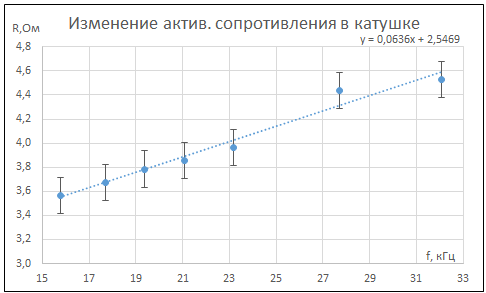
\includegraphics[width = 0.7 \textwidth]{RL}
	\caption{\footnotesize
	Зависимость активного сопротивления потерь $ R_L $ катушки от частоты сигнала (резонанс).
	}
	\label{RL}
\end{figure}

Данная картина наблюдается в следствие того, что с увеличением частоты также возрастает
реактивное сопротивление у катушки индуктивности. Импеданс для $ L $:
$ Z_L = i \: \omega L $

\end{enumerate}

\vspace{-0.7cm}

\subsection*{Погрешности}

\vspace{-0.3cm}

\ \ Погрешности измерений рассматривались параллельно с нахождением каждой из величин.
Все же отметим некоторые из них.\\
Конечно, главным источником ошибок во многих работах является человеческий фактор:
в данной работе -- снятие показаний с осциллографа. Приборные погрешности достаточно малы:
у вольтметра -- 1 мВ, для частоты сигнала -- 1Гц; тогда как измерения превышают их
в сотни раз.\\
Все же даже погрешности измерений на осциллографе меньше, чем случайные, которые рассчитаны
в таблице \ref{tabFinal}.\\
Окончательные результаты для ошибок также находятся в таблице \ref{tabFinal}.

\vspace{-0.1cm}

\section*{Итоги}

\vspace{-0.1cm}

В данной работе исследован резонанс напряжений в последовательном колебательном контуре
с изменяемой емкостью. Также получили АЧХ и ФЧХ, определили основные параметры контура
(таблица \ref{tabFinal}).\\
Нашли добротности для контуров с емкостями $ C_2 \ и \ C_6 $ тремя разными способами.
Учитывая погрешности, результаты совпадают.

\begin{table}[H]
	\centering
	\begin{tabular}{|c|c|c|c|}
		\hline
				& Теоретически		& АЧХ				& ФЧХ 				\\ \hline
		$ Q_2 $	& $ 21,9 \pm 0,1 $	& $ 21,3 \pm 0,9 $	& $ 22,2 \pm 1,0 $	\\
		$ Q_6 $	& $ 15,1 \pm 0,1 $	& $ 14,6 \pm 0,4 $	& $ 14,7 \pm 0,4 $	\\ \hline
	\end{tabular}
	\caption{\footnotesize 
	Добротности колебательных контуров с конденсаторами $ C_2 \ и \ C_6 $
	}
	\label{result}
\end{table}

\end{document}